\documentclass[10pt]{article}         %% What type of document you're writing.
\usepackage{graphicx}
\usepackage{hyperref}
\usepackage[dvipsnames]{xcolor}

%%%%% Preamble

%% Packages to use

\usepackage{amsmath,amsfonts,amssymb}   %% AMS mathematics macros

%% Title Information.

\title{Amazon Data Model}
\author{Leonardo Martinez}
%% \date{29 sep 2020}           %% By default, LaTeX uses the current date

%%%%% The Document

\begin{document}

\maketitle

\begin{abstract}
This document implements the Amazon Data Model.
\end{abstract}

\section{Data Model Desciption}


\textcolor{red}{Proveedores} de Amazon ( \textcolor{green}{codigo, nombre, rating} )\\

\textcolor{red}{Productos} ( \textcolor{green}{codigo, nombre, descripcion, precio, diasentrega, categoria,empresa de reparto} )
\\
\textcolor{red}{Clientes}( \textcolor{green}{ codigo, usuario, password, nombre, direccion} )\\

Los clientes \textcolor{yellow}{compran} n producto

Los proveedores \textcolor{yellow}{surten} n productos


Amazon ...
\section{E-R Model}
\begin{figure}[b]
     \includegraphics[scale=0.4]{amazon_er.png}
     \caption{Amazon E-R Model}
\end{figure}

\section{Relation Model}
\begin{figure}[b]
     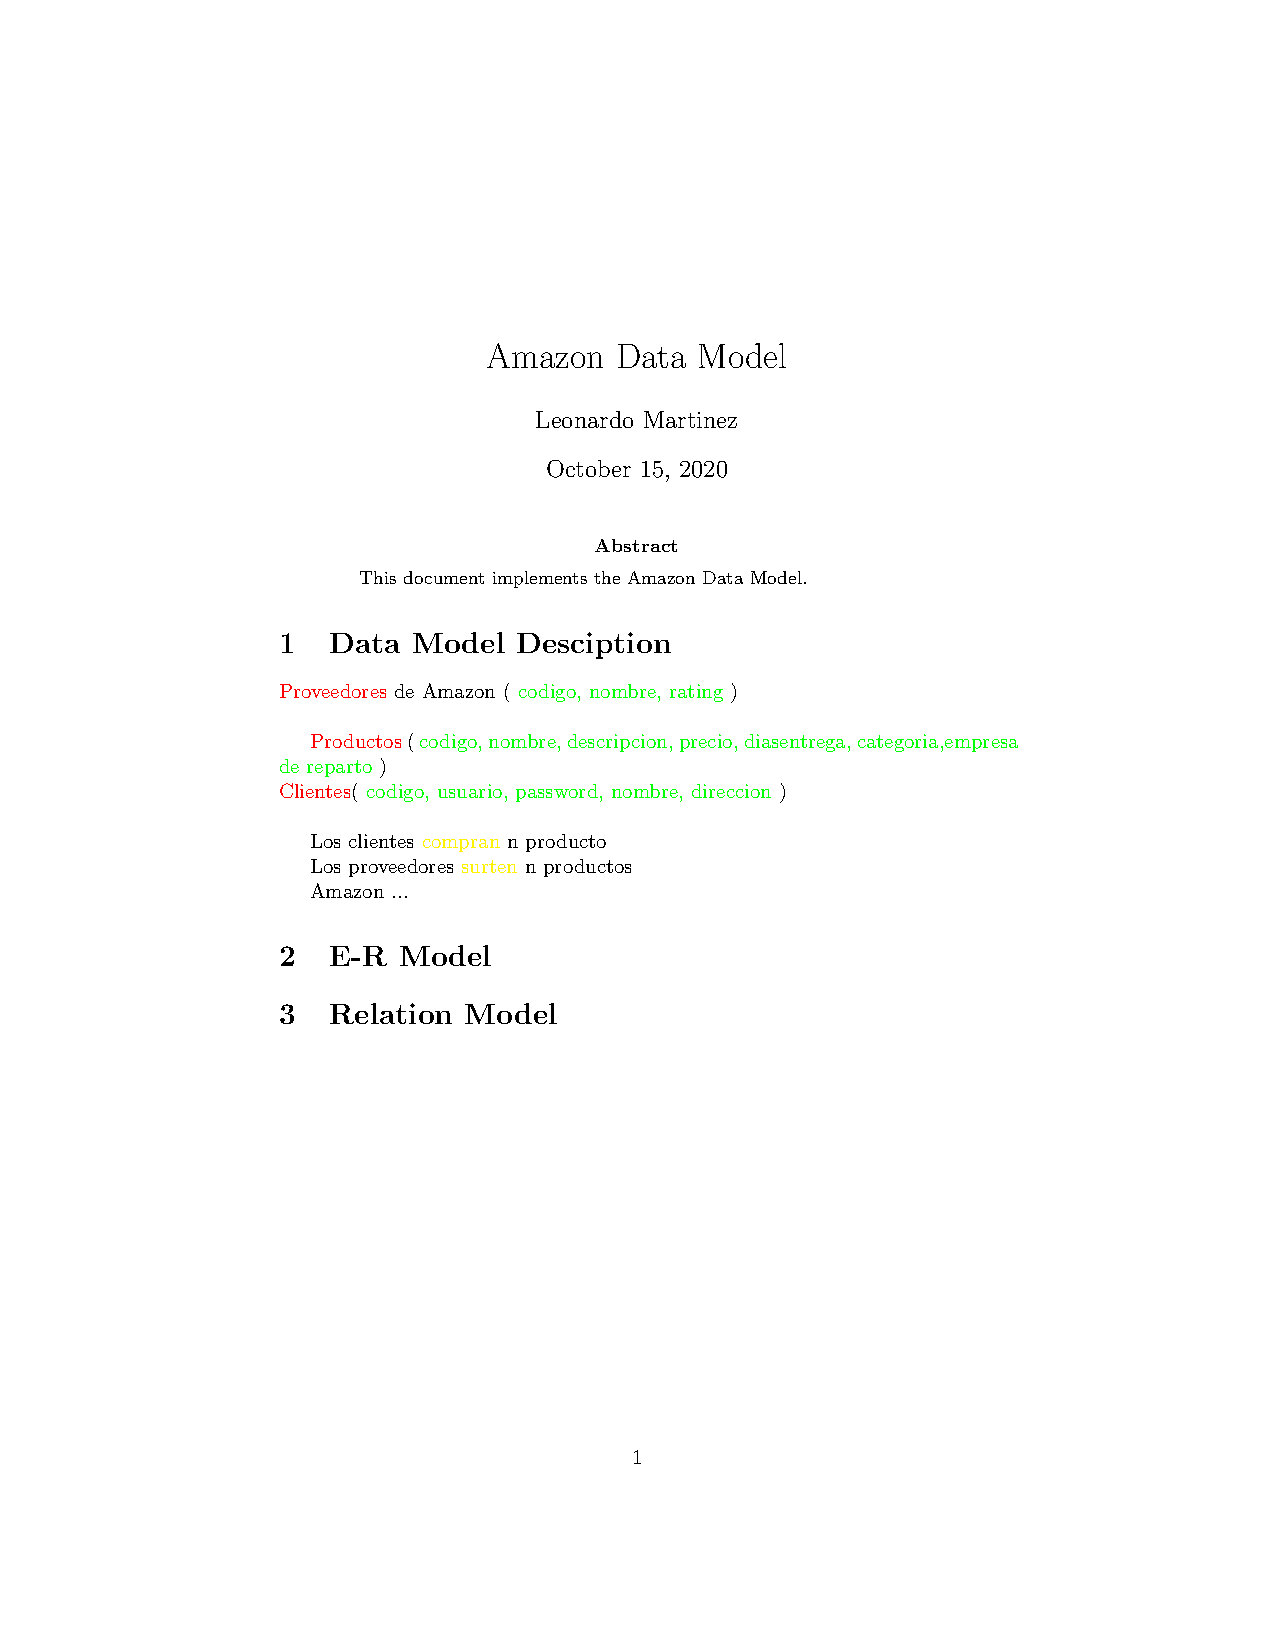
\includegraphics[scale=0.4]{amazon_relation_model.png}
     \caption{Amazon Relation Model}
\end{figure}

\section{STEPS}
\begin{enumerate}
	\item
	ssh -i leonardodmm leonardodmm@104.198.244.0
	\item
	sudo -u postgres createdb leonardodmm\_amazon;
	\item
	sudo -u postgres psql;
	\item
	\textbackslash connect leonardoddmm\_amazon;
	\item
	create table provedores(codigoprov int,rating int,nombre varchar(200));
	\item
	alter table provedores add constraint pk\_codigoprov primary key(codigoprov);
	\item
	create table cliente(codigocliente int,nombre varchar(80),apellidopat varchar(30),apellidomat varchar(30),password varchar(30),usuario varchar(40),codigopost varchar(10),estado varchar(100),colonia varchar (100),calleyav varchar(120));
	\item
	alter table cliente add constraint pk\_codigocliente primary key(codigocliente);
	\item
	create table prodcategoria(codcategoria int,clasificacion varchar(200));
	\item
	alter table prodcategoria  add constraint pk\_codcategoria primary key(codcategoria);
	\item
	create table proempresarep(codempresarep int,paqueteria varchar(200));
	\item
	alter table proempresarep add constraint pk\_codeempresarep primary key(codempresarep);
	\item
	create table productos(codigoProd int,codcategoria int,codempresa int,nombre varchar(80),descripcion varchar(200),precio float,diasentrega varchar);
	\item
	alter table productos add constraint codigoprod primary key(codigoprod);
	\item
	alter table productos add constraint fk\_codcategoria foreign key(codcategoria)
references prodcategoria(codcategoria);
	\item
	alter table productos add constraint fk\_codempresa foreign key(codempresa) references proempresarep(codempresarep);
	\item
	create table provedorproducto(codigoprov int,codprod int);
	\item
	alter table provedorproducto add constraint pk\_codigoprov\_codprod primary key (codigoprov,codprod);
	\item
	alter table provedorproducto add constraint fk\_codigoprov foreign key(codigoprov) references provedores(codigoprov);
	\item
	alter table provedorproducto add constraint fk\_codprod foreign key(codprod) references productos(codigoprod);
	\item
	create table clienteproducto(codcliente int,codigoprod int);
	\item
	alter table clienteproducto add constraint pk\_codcliente\_codigoprod primary key(codcliente,codigoprod);
	\item
	alter table clienteproducto add constraint fk\_codcliente foreign key(codcliente) references cliente(codigocliente);
	\item
	alter table clienteproducto add constraint fk\_codigoprod foreign key(codigoprod) references productos(codigoprod);

	
\end{enumerate}
\end{document}
